\documentclass[bst/sn-nature]{sn-jnl}
\usepackage{graphicx}%
\usepackage{multirow}%
\usepackage{amsmath,amssymb,amsfonts}%
\usepackage{amsthm}%
\usepackage{mathrsfs}%
\usepackage[title]{appendix}%
\usepackage{xcolor}%
\usepackage{textcomp}%
\usepackage{manyfoot}%
\usepackage{booktabs}%
\usepackage{algorithm}%
\usepackage{algorithmicx}%
\usepackage{algpseudocode}%
\usepackage{listings}%
\usepackage{multicol} % Add this package
\usepackage{hhline}
\usepackage{colortbl}
\usepackage{caption}
\usepackage{longtable}
\usepackage{lipsum}
\usepackage{makecell}
\usepackage{booktabs} % Add this in your preamble
\usepackage{array} 
\usepackage[table]{xcolor}  % In your preamble
\usepackage{booktabs} 
\geometry{
    left=0.8cm,
    right=0.8cm,
    top=2cm,
    bottom=4cm,
}

\begin{document}

\title[Article Title]{Predicting Postoperative Complications in Laparoscopic General Surgery Using Machine and Deep Learning: A Classification Approach}

\author*[1]{\fnm{Tyler} \sur{Wallett}}\email{twallett@gwu.edu}

\author[2]{\fnm{Amir} \sur{Jafari}}\email{ajafari@gwu.edu}

\author[3]{\fnm{Xi} \sur{Qian}}\email{qianxi@gwu.edu}

\author[4]{\fnm{Timur} \sur{Abdygulov}}\email{timur.abdygulov@gwu.edu}

\author[5]{\fnm{Xiao} \sur{Qi}}\email{xiao.qi@tamu.edu}

\author[6]{\fnm{Neda} \sur{Nourshamsi}}\email{n.nourshamsi@ieee.org}

\author[7]{\fnm{Jevaughn} \sur{Davis}}\email{jdavis26@gwu.edu}

\author[8]{\fnm{Gupta} \sur{Puneet}}\email{guptap14@gwu.edu}
 
\affil[1,2,3,4]{\orgdiv{Data Science}, \orgname{The George Washington University}, \city{Washington},\state{ D.C}}

\affil[5]{\orgname{Texas A\&M University}, \city{College Station}, \state{Texas}}

\affil[6]{\orgname{Mu-Del Electronics}, \city{Industry}, \state{Virginia}}

\affil[7,8]{\orgdiv{Department of Anesthesiology and Critical Care Medicine}, \orgname{The George Washington University}, \city{Washington}, \state{D.C}}

\abstract{\quad Postoperative complications following laparoscopic general surgery contribute significantly to patient morbidity, mortality, and healthcare costs. This study develops and evaluates machine learning and deep learning models to predict six critical postoperative complications: cardiac arrest, myocardial infarction, pulmonary embolism, reintubation, pneumonia, and failure to wean from ventilatory support. Using a deidentified dataset of 210,349 patient records, we implemented a comprehensive classification pipeline to address the substantial class imbalance inherent in surgical complications data. The pipeline incorporated preprocessing techniques, synthetic minority oversampling, and systematic evaluation of machine learning algorithms and deep learning architectures. Model performance was assessed using Area Under the Curve (AUC) and recall metrics, with particular emphasis on maximizing the detection of true positive cases given the clinical importance of early intervention. To complement these metrics Receiver Operator Characteristic (ROC) visualizations and confusion matrices were provided. We compared the performance of different models across the six complications and identified which approaches were most effective for specific adverse outcomes. Our findings provide insights into the relative value of model complexity versus interpretability in clinical prediction tasks and highlight important considerations for the implementation of predictive analytics in surgical care. This research contributes to the advancement of predictive analytics in postoperative care and offers practical recommendations for clinical integration to improve surgical outcomes through early intervention and optimized resource allocation.}

\keywords{Neural Networks, Supervised Learning, Postoperative Complications}

\maketitle

\begin{multicols}{2}

%%%%%%%%%%%%%%%%%%%%%%%%%%%%%%%%%%%%%%%%%%%%%%%%%
\section{Introduction}
\begin{table*}[b]
\centering
\caption{Input Features Data Dictionary.}
\label{tab:input_feature_dict}
\begin{tabular}{ll}
\toprule
\textbf{Name of Feature} & \textbf{Description of Feature} \\
\midrule
\rowcolor{gray!10} Age & Patient's age \\
Sex & Patient's biological sex (Male, Female, Non-binary) \\
\rowcolor{gray!10} Race & Patient's race categorization (White, African American, Unknown, Other, Asian, Mixed) \\
BMI & Patient's Body Mass Index \\
\rowcolor{gray!10} Hospital Status & Patient's hospital status (Inpatient, Outpatient) \\
ASA Classification & ASA physical status classification (No Disturb, Mild Disturb, Severe Disturb, Life Threat) \\
\rowcolor{gray!10} CPT & Current Procedural Terminology code \\
Diabetes & Patient's diabetes status (No, Yes) \\
\rowcolor{gray!10} Smoke & Patient's smoking status (No, Yes) \\
Functional Health Status & Patient's pre-operative functional health status (Independent, Dependent) \\
\rowcolor{gray!10} History Pulmonary Disease & Patient's history of chronic obstructive pulmonary disease (No, Yes) \\
Ascites & Presence of ascites in patient (No, Yes) \\
\rowcolor{gray!10} History Congestive Heart Failure & Patient's history of congestive heart failure (No, Yes) \\
Hypertension Medication & Patient requires hypertension medication (No, Yes) \\
\rowcolor{gray!10} Dialysis & Patient's dialysis for renal failure (No, Yes) \\
Disseminated Cancer & Patient's disseminated cancer (No, Yes) \\
\rowcolor{gray!10} Steroid & Patient's chronic corticosteroid use (No, Yes) \\
Transfusion & Patient's blood transfusion status (No, Yes) \\
\bottomrule
\end{tabular}
\end{table*}

\quad Postoperative complications after general laparoscopic surgery represent significant challenges to patient recovery, healthcare resource utilization, and overall surgical outcomes. Despite advances in minimally invasive surgical techniques, patients continue to experience serious adverse events such as cardiac arrest, myocardial infarction, pulmonary embolism, reintubation, pneumonia, and failure to wean from ventilatory support. These complications not only impact patient morbidity and mortality, but also substantially increase healthcare costs through extended hospital stays, readmissions, and additional interventions\cite{challenges3}.

Early prediction of such complications remains a critical yet challenging aspect of perioperative care. Traditional risk assessment tools often rely on simplified scoring systems with limited discriminative ability in diverse patient populations\cite{challenges1}\cite{challenges2}. However, recent advances in machine learning and deep learning methodologies offer promising alternatives for developing more accurate and personalized risk prediction models by leveraging the wealth of preoperative patient data available in modern electronic health records\cite{promises1}\cite{promises2}\cite{promises3}.

The potential of artificial intelligence in healthcare has been validated through widespread applications across medical domains. The COVID-19 pandemic accelerated AI adoption, demonstrating effectiveness in medical diagnosis, prognosis, and treatment optimization\cite{covid_ai_survey}. Hybrid CNN-transformer architectures have achieved superior performance in complex medical segmentation tasks\cite{hybrid_cnn_transformer}, while advanced data augmentation frameworks address class imbalance challenges prevalent in medical datasets\cite{medical_augmentation}. Specialized neural architectures, such as point tracking networks in cardiac imaging\cite{manet_cardiac}, illustrate the potential for task-specific models that capture complex patient-outcome relationships, providing methodological foundations for perioperative risk assessment.

This study develops and evaluates predictive models for six clinically significant postoperative complications following general laparoscopic surgery. Using a deidentified dataset, we employ machine learning algorithms and deep neural networks to address class imbalance and complex relationships within surgical outcome data.

Our research makes several key contributions. First, we present a systematic comparison of multiple predictive modeling approaches across multiple postoperative complications, providing insights into which algorithms perform best for specific adverse outcomes. Second, we address class imbalance through targeted oversampling techniques. Third, we evaluate models on both discriminative performance metrics (AUC) and clinically relevant measures (recall, specificity), directly impacting practical utility in surgical settings.

The paper is organized as follows: Section 2 describes the dataset and features; Section 3 presents exploratory data analysis; Section 4 details our methodology; Section 5 reports experimental results; Section 6 discusses clinical implications and practical recommendations\cite{promises4}; Section 7 concludes with contributions and future research directions. This work aims to enable earlier interventions, optimize resource allocation, and improve patient outcomes after laparoscopic surgery.

%%%%%%%%%%%%%%%%%%%%%%%%%%%%%%%%%%%%%%%%%%%%%%%%%
\section{Dataset}

\begin{table*}[t]
\centering
\caption{Distribution of Targets Summary.}
\label{tab:target_distribution_summary}
\rowcolors{2}{gray!10}{white}  % Starts from the first data row
\begin{tabular}{llcc}
\toprule
\textbf{Name of Variable} & \textbf{Class Description} & \textbf{Count} & \textbf{Percentage (\%)} \\
\midrule
Cardiac Arrest & No Complication      & 210\,105 & 99.88 \\
               & Cardiac Arrest        & 244     & 0.12  \\
Myocardial Infarction & No Complication      & 209\,893 & 99.78 \\
                      & Myocardial Infarction & 456     & 0.22  \\
Pulmonary Embolism & No Complication       & 209\,845 & 99.76 \\
                   & Pulmonary Embolism    & 504     & 0.24  \\
Reintubation & No Complication        & 209\,858 & 99.77 \\
             & Unplanned Intubation   & 491     & 0.23  \\
Pneumonia & No Complication           & 209\,147 & 99.43 \\
          & Pneumonia                 & 1\,202   & 0.57  \\
Failure to Wean from Ventilator & No Complication        & 209\,994 & 99.83 \\
                                & Ventilator $>$ 48 Hours & 355     & 0.17  \\
\bottomrule
\end{tabular}
\end{table*}


\quad This study was deemed exempt from IRB review as all data used were deidentified and publicly available. The dataset comprised 210,349 patient records from the ACS NSQIP Participant Use Data File, a national registry that includes perioperative data from more than 600 hospitals in the United States. Each record represents a unique laparoscopic general surgery case and includes preoperative clinical and demographic features used to predict postoperative complications occurring within 30 days of surgery.

The dataset includes 19 input features, of which only two variables (Age and BMI) are continuous; the remaining features are categorical. These features were selected based on their known or potential clinical relevance to surgical outcomes\cite{features}. Demographic variables such as age, sex, and race can influence physiological responses to surgery and healing rates. Comorbid conditions such as diabetes, pulmonary disease, heart failure, and cancer are widely recognized risk factors for poor postoperative outcomes\cite{comorbidity}. Lifestyle factors such as smoking and the need for hypertension medications provide additional context to the overall health status of the patient. Information about the procedure, such as the CPT code and hospital status, offers insight into the complexity and setting of the surgical intervention. Inclusion of the ASA physical status classification and functional health status adds an important layer of preoperative risk stratification. A detailed summary of these features is presented in Table~\ref{tab:input_feature_dict}.

The target variables represent six clinically significant postoperative complications: cardiac arrest, myocardial infarction, pulmonary embolism, unplanned reintubation, pneumonia, and failure to wean from a ventilator. These complications were selected due to their association with increased morbidity, extended hospital stays, intensive care utilization, and mortality. Early and accurate prediction of such adverse outcomes is critical for surgical risk assessment and perioperative planning. Each outcome is framed as a binary classification task and exhibits substantial class imbalance, with complication rates ranging from 0.12\% to 0.57\%. A summary of the distributions of the target variables is provided in Table~\ref{tab:target_distribution_summary}.

%%%%%%%%%%%%%%%%%%%%%%%%%%%%%%%%%%%%%%%%%%%%%%%%%
\section{Exploratory Data Analysis}

\begin{figure*}
    \centering
    
\includegraphics[width=0.65\linewidth]{imgs/correlation-matrix.pdf}
    \caption{Correlation Matrix.}
    \label{fig:pipeline}
\end{figure*}

\quad To examine the degree of association between categorical variables in our dataset, we employed the Cramer's V coefficient, a measure particularly suited for nominal data. Cramer's V is calculated using the following formula:

\begin{equation}
V = \sqrt{\frac{\chi^2/n}{\min(k-1, r-1)}}
\end{equation}

where $\chi^2$ is the Pearson chi-square statistic, $n$ is the total sample size, $k$ is the number of columns, and $r$ is the number of rows in the contingency table. The coefficient ranges from 0 (no association) to 1 (perfect association), providing a standardized measure of the size of the effect. Since Cramer's V is particularly useful in identifying correlation coefficients between two categorical values, we discretized Age and BMI by simply rounding each value.

Our Cramer's V correlation matrix revealed several clinically significant relationships between patient characteristics and comorbidities. Age emerged as a significant factor, showing a strong association with hypertension (V = 0.48) and moderate associations with ASA classification (V = 0.26). The ASA physical status classification demonstrated substantial correlations with hypertension (V = 0.38), diabetes (V = 0.26), and history of congestive heart failure (V = 0.25), reinforcing its role as an integrated measure of surgical risk. The correlation between diabetes and hypertension (V = 0.31) confirms their frequent co-occurrence. BMI showed moderate associations with ASA classification (V = 0.19) and diabetes (V = 0.14), highlighting the relationship between obesity and cardiometabolic conditions. Inpatient/outpatient status correlated with ASA classification (V = 0.20), indicating that higher-risk patients typically undergo inpatient procedures. Cardiopulmonary connections were evident between pulmonary disease, ASA classification (V = 0.17), and congestive heart failure (V = 0.13). In particular, demographic factors such as sex and race showed relatively weak associations with most clinical variables, suggesting that specific comorbidities may be more direct predictors of surgical outcomes than demographics alone.

%%%%%%%%%%%%%%%%%%%%%%%%%%%%%%%%%%%%%%%%%%%%%%%%%
\section{Methodology}

\quad This study presents a comprehensive machine learning and deep learning pipeline designed to classify postoperative complications in six highly unbalanced target variables. The complete implementation of the methodology is publicly available\footnote{GitHub Link: \href{https://github.com/twallett/research/tree/main/2025/postoperative-risk-prediction}{Link}}.

The general workflow of the classification pipeline is illustrated in Figure~\ref{fig:pipeline}. The process begins with the dataset being partitioned into training (80\%) and testing (20\%) subsets to facilitate robust evaluation and generalization of the models. Following this, the training data is passed through a preprocessing stage, where missing values are handled, categorical variables are encoded, and feature scaling is applied.

Subsequently, given the significant imbalance in postoperative complication outcomes, oversampling techniques are used in training data to improve the representation of minority classes and improve classifier performance.

The study evaluates a wide range of models, including machine learning algorithms such as Logistic Regression, Gaussian Naive Bayes, Decision Trees, Random Forest, XGBoost, and K-Nearest Neighbors, as well as deep learning architectures including 2, 4, and 8 layer Multi-Layered Perceptrons (MLPs) and Convolutional Neural Networks (CNNs). Hyperparameter optimization is performed using grid or randomized search with cross validation of 3 for classical models, and Keras Tuner\cite{kerastuner} with maximum trials of 3 for neural network architectures.

Model performance is assessed using multiple metrics, with a strong emphasis on recall to capture as many true positive complication cases as possible. These metrics include AUC, recall, ROC visualizations, and confusion matrices. All performance metrics are reported on the test set to ensure an unbiased evaluation.

%%%%%%%%%%%%%%%%%%%%%%%%%%%%%%%%%%%%%%%%%%%%%%%%%
\subsection{Data Preprocessing}

\begin{figure*}
    \centering
    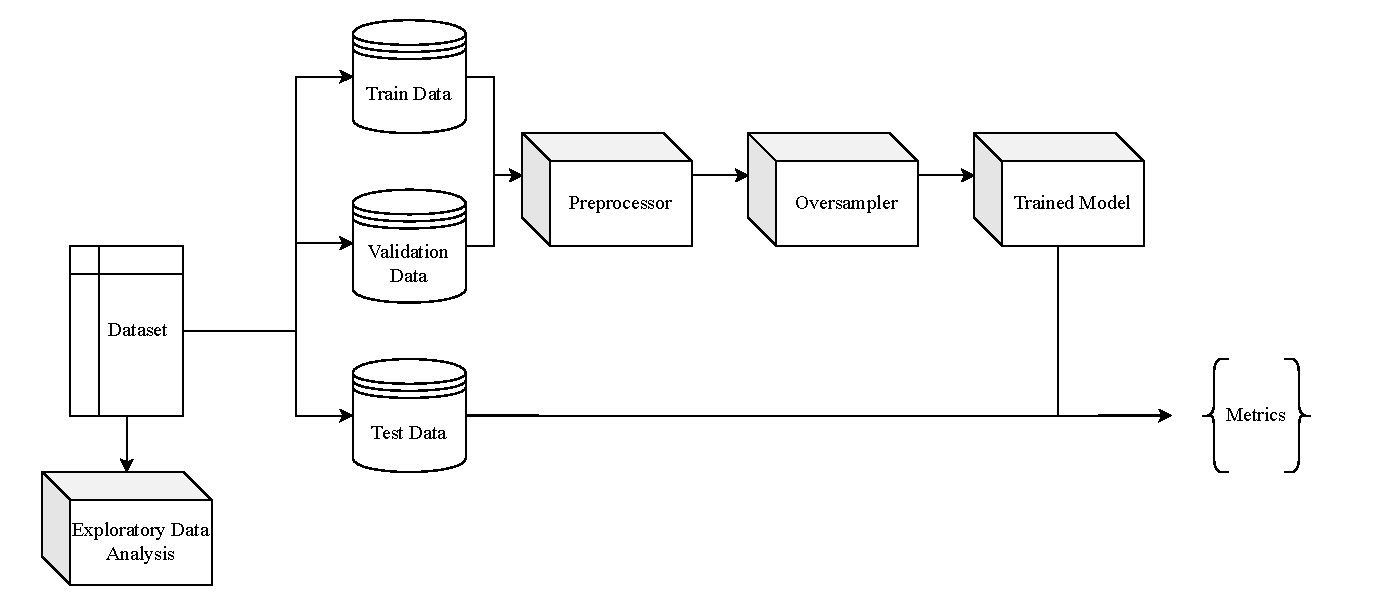
\includegraphics[width=\linewidth]{imgs/ML-Pipeline.drawio.pdf}
    \caption{Machine and Deep Learning Pipeline.}
    \label{fig:pipeline}
\end{figure*}

\quad A systematic preprocessing pipeline was implemented to ensure the dataset was appropriately formatted for downstream machine learning and deep learning tasks. Categorical variables were encoded using \texttt{LabelEncoder}, transforming string-based labels into numeric values. This encoding was applied iteratively to all input features with object datatypes.

Continuous features—specifically Age and BMI—were standardized using \texttt{StandardScaler} to normalize their distributions. The scaler was fit exclusively on the training data and subsequently applied to the validation and test sets, preserving the integrity of the model evaluation process.

The preprocessing was performed independently for each clinical outcome to support the one-vs-rest classification framework. This approach ensured that each binary classification task was handled in isolation and prepared the dataset for the oversampling procedures.

%%%%%%%%%%%%%%%%%%%%%%%%%%%%%%%%%%%%%%%%%%%%%%%%%
\subsection{Oversampling}

\quad To address the significant class imbalance in our dataset (see Table~\ref{tab:target_distribution_summary}), we use the Synthetic Minority Over-sampling Technique\cite{smote} (SMOTE) using the \texttt{imblearn\cite{imblearn}} library. Although our feature set consisted of 2 continuous and 17 categorical features, we chose SMOTE over SMOTE for Nominal and Continuous features (SMOTENC). Although SMOTENC is specifically designed to handle mixed-type data by treating categorical variables differently during sample generation, we found that SMOTE led to superior model performance in our experiments. This improvement is likely due to the ability of SMOTE to generate smoothly interpolated synthetic samples within the minority class, aiding the model in learning more generalizable decision boundaries, even at the cost of disregarding the categorical nature of some features. After applying SMOTE, each binary target variable in the training set exhibited a perfectly balanced distribution, with exactly 50\% of samples belonging to the complication class and 50\% to the no complication class. This choice was empirically validated through 3-fold cross-validation, where models trained on SMOTE-balanced data consistently outperformed those trained on data balanced using SMOTENC across key performance metrics.

%%%%%%%%%%%%%%%%%%%%%%%%%%%%%%%%%%%%%%%%%%%%%%%%%
\subsection{Machine Learning}

\quad Machine learning (ML) models form the basis for supervised learning algorithms. These models are widely used for classification tasks because of their simplicity, interpretability, and effectiveness in various real-world scenarios. In this section, we explore several classical models available through the popular machine learning library \texttt{scikit-learn\cite{sklearn_api}} (sklearn), which is a powerful toolkit for building and evaluating predictive models.

The models discussed include linear models like Logistic Regression, probabilistic models such as Gaussian Naive Bayes, tree-based methods with Decision Trees, and ensemble methods like Random Forest and XGBoost. These algorithms vary in their approach to learning patterns from data but share the common goal of making accurate predictions. Each model's core methodology, mathematical formulation, and common use cases are summarized in the following subsections.

\begin{table*}
    \centering
    \begin{tabular}{|l|c|c|c|c|c|c|}
    \hline
    \textbf{Model} & \textbf{Target} & \textbf{$k$} & \textbf{Criterion} & \textbf{Max Depth} & \textbf{Learning Rate} & \textbf{\# Estimators} \\
    \hline
    \rowcolor[gray]{0.9} Decision Tree & Cardiac Arrest & - & entropy & 20 & - & - \\
    Decision Tree & Myocardial Infarction & - & gini & 20 & - & - \\
    \rowcolor[gray]{0.9} Decision Tree & Pulmonary Embolism & - & entropy & 20 & - & - \\
    Decision Tree & Reintubation & - & gini & 20 & - & - \\
    \rowcolor[gray]{0.9} Decision Tree & Pneumonia & - & gini & 20 & - & - \\
    Decision Tree & Failure to Wean & - & gini & 20 & - & - \\
    \rowcolor[gray]{0.9} Random Forest & Cardiac Arrest & - & - & 30 & - & 300 \\
    Random Forest & Myocardial Infarction & - & - & 30 & - & 300 \\
    \rowcolor[gray]{0.9} Random Forest & Pulmonary Embolism & - & - & 30 & - & 300 \\
    Random Forest & Reintubation & - & - & 30 & - & 300 \\
    \rowcolor[gray]{0.9} Random Forest & Pneumonia & - & - & 30 & - & 300 \\
    Random Forest & Failure to Wean & - & - & 30 & - & 300 \\
    \rowcolor[gray]{0.9} XGBoost & Cardiac Arrest & - & - & 20 & 0.10 & 100 \\
    XGBoost & Myocardial Infarction & - & - & 10 & 0.01 & 100 \\
    \rowcolor[gray]{0.9} XGBoost & Pulmonary Embolism & - & - & 10 & 0.01 & 100 \\
    XGBoost & Reintubation & - & - & 10 & 0.01 & 100 \\
    \rowcolor[gray]{0.9} XGBoost & Pneumonia & - & - & 10 & 0.01 & 100 \\
    XGBoost & Failure to Wean & - & - & 10 & 0.01 & 100 \\
    \rowcolor[gray]{0.9} K-Nearest Neighbors & Cardiac Arrest & 11 & manhattan & - & - & - \\
    K-Nearest Neighbors & Myocardial Infarction & 11 & manhattan & - & - & - \\
    \rowcolor[gray]{0.9} K-Nearest Neighbors & Pulmonary Embolism & 11 & manhattan & - & - & - \\
    K-Nearest Neighbors & Reintubation & 11 & manhattan & - & - & - \\
    \rowcolor[gray]{0.9} K-Nearest Neighbors & Pneumonia & 9 & manhattan & - & - & - \\
    K-Nearest Neighbors & Failure to Wean & 11 & manhattan & - & - & - \\
    \hline
    \end{tabular}
    \caption{Summary of Machine Learning Model Hyperparameters.}
    \label{tab:classical_hyperparams}
\end{table*}

%%%%%%%%%%%%%%%%%%%%%%%%%%%%%%%%%%%%%%%%%%%%%%%%%
\subsubsection{Logistic Regression\cite{nndesign}}

\quad Logistic regression is a linear statistical model used for binary classification. It begins by computing a linear combination of the input features: \\

\begin{center}
    $n = \mathbf{w}^\top \mathbf{p} + b$ \vspace{0.3cm}
\end{center}

where $\mathbf{p}$ is the input vector, $\mathbf{w}$ is the weight vector, and $b$ is the bias term. This scalar output $n$ is then passed through the sigmoid activation function: \\

\begin{center}
    $f(n) = \frac{1}{1 + e^{-n}}$ \vspace{0.3cm}
\end{center}

which maps the result to a value between 0 and 1. The final prediction is then computed as: \\ 

\begin{center}
    $a = f(\mathbf{w}^\top \mathbf{p} + b)$ \vspace{0.3cm}
\end{center}

where $a$ represents the model's estimated probability that the input $\mathbf{p}$ belongs to the positive class. This probability can be thresholded to produce a binary decision. Logistic regression is widely used due to its simplicity, interpretability, and effectiveness in linearly separable scenarios.

%%%%%%%%%%%%%%%%%%%%%%%%%%%%%%%%%%%%%%%%%%%%%%%%%
\subsubsection{Gaussian Naive Bayes\cite{naivebayes}}

\quad Gaussian Naive Bayes is a generative classification algorithm that models each class-conditional feature distribution as Gaussian and assumes that features are conditionally independent given the class. The prior probability of each class $c_i$ is computed as: \\ 

\begin{center}
    $P(c_{i}) = \frac{\text{number of samples in class} \ c_{i}}{ \text{total number of samples}}$ \quad for $i = 1, 2, \dots, C$ \vspace{0.3cm}
\end{center}

where $C$ is the total number of classes. For each feature $n$ and class $c_i$, the likelihood is modeled using the Gaussian (normal) distribution: \\

\begin{center}
    $P(\mathbf{p}_{n}|c_i) = \frac{1}{\sqrt{2 \pi \sigma^{2}_{n,i}}} \exp\left(-\frac{(\mathbf{p}_n - \mu_{n,i})^2}{2 \sigma^{2}_{n,i}}\right)$ \vspace{0.3cm}
\end{center}

where $\mu_{n,i}$ and $\sigma^2_{n,i}$ are the mean and variance of feature $n$ in class $c_i$, respectively, and $n = 1, 2, \dots, N$ for $N$ features. The posterior probability of a class given the input vector is then computed using Bayes’ theorem: \\ 

\begin{center}
    $P(c_i|\mathbf{p}_{n}) = P(c_i) \prod^{N}_{n=1} P(\mathbf{p}_{n}|c_i)$ \vspace{0.3cm}
\end{center}

where the independence assumption allows the likelihoods to be multiplied across features. Finally, the predicted class is selected as the one with the highest posterior probability: \\

\begin{center}
    $a = \arg\max_c P(c_i|\mathbf{p}_{n})$ \vspace{0.3cm}
\end{center}

Gaussian Naive Bayes is especially effective for high-dimensional problems, offering a simple yet powerful probabilistic framework.

\begin{table*}
    \centering
    \small % Reduce font size
    \setlength{\tabcolsep}{2pt}
    \begin{tabular}{|l|c|c|c|c|c|c|c|c|c|}
    \hline
    \textbf{Model} & \textbf{Target} & \textbf{Units 1} & \textbf{Units 2} & \textbf{Units 3} & \textbf{Units 4} & \textbf{Dropout 1} & \textbf{Dropout 2} & \textbf{Dropout 3} & \textbf{Learning Rate} \\
    \hline
    \rowcolor[gray]{0.9} 2 Layer & Cardiac Arrest & 40 & - & - & - & - & - & - & 0.01 \\
    4 Layer & Cardiac Arrest & 96 & 48 & 8 & - & - & - & 0.3 & 0.01 \\
    \rowcolor[gray]{0.9} 8 Layer & Cardiac Arrest & 192 & 32 & 16 & 16 & 0.2 & 0.1 & 0.1 & 0.01 \\
    2 Layer & Myocardial Infarction & 104 & - & - & - & - & - & - & 0.001 \\
    \rowcolor[gray]{0.9} 4 Layer & Myocardial Infarction & 96 & 64 & 8 & - & - & - & 0.4 & 0.01 \\
    8 Layer & Myocardial Infarction & 192 & 128 & 32 & 24 & 0.2 & 0.3 & 0.1 & 0.001 \\
    \rowcolor[gray]{0.9} 2 Layer & Pulmonary Embolism & 72 & - & - & - & - & - & - & 0.001 \\
    4 Layer & Pulmonary Embolism & 64 & 64 & 16 & - & - & - & 0.1 & 0.001 \\
    \rowcolor[gray]{0.9} 8 Layer & Pulmonary Embolism & 192 & 96 & 48 & 16 & 0.2 & 0.4 & 0.2 & 0.001 \\
    2 Layer & Reintubation & 8 & - & - & - & - & - & - & 0.01 \\
    \rowcolor[gray]{0.9} 4 Layer & Reintubation & 128 & 64 & 8 & - & - & - & 0.2 & 0.0001 \\
    8 Layer & Reintubation & 64 & 64 & 16 & 24 & 0.1 & 0.1 & 0.1 & 0.001 \\
    \rowcolor[gray]{0.9} 2 Layer & Pneumonia & 72 & - & - & - & - & - & - & 0.01 \\
    4 Layer & Pneumonia & 128 & 16 & 8 & - & - & - & 0.5 & 0.001 \\
    \rowcolor[gray]{0.9} 8 Layer & Pneumonia & 192 & 64 & 32 & 24 & 0.1 & 0.2 & 0.1 & 0.01 \\
    2 Layer & Failure to Wean & 40 & - & - & - & - & - & - & 0.01 \\
    \rowcolor[gray]{0.9} 4 Layer & Failure to Wean & 128 & 48 & 16 & - & - & - & 0.2 & 0.001 \\
    8 Layer & Failure to Wean & 256 & 32 & 64 & 8 & 0.1 & 0.3 & 0.1 & 0.001 \\
    \hline
    \end{tabular}
    \caption{Summary of MLP Model Hyperparameters.}
    \label{tab:mlp_hyperparams}
\end{table*}

%%%%%%%%%%%%%%%%%%%%%%%%%%%%%%%%%%%%%%%%%%%%%%%%%
\subsubsection{Decision Tree\cite{decisiontrees}}

\quad Decision trees are non-parametric supervised learning models used for classification tasks. At each node in the tree, the algorithm evaluates a splitting criterion to determine the quality of a potential split. One common criterion is the Gini impurity, calculated as: \\ 

\begin{center}
    $\text{Gini}(\text{node}) = 1 - \sum^{C}_{c=1} p^2_c$ \vspace{0.3cm}
\end{center}

where $p_c$ is the proportion of samples belonging to class $c$ at a given node and $C$ is the total number of classes. Another widely used criterion is information gain, which is derived from entropy: \\

\begin{center}
    $\text{Entropy}(\text{node}) = - \sum^{C}_{c=1} p_c \log_2 p_c$ \vspace{0.3cm}
\end{center}

Entropy measures the level of uncertainty or disorder in the class distribution at a node. To evaluate the effectiveness of a split, the change in impurity for a particular criterion is computed as: \\ 

\begin{center}
    $\Delta I(\text{node}) = I(\text{node}_{\text{parent}}) - \left(\frac{\text{left samples}}{\text{total samples}} I(\text{node}_{\text{left}}) + \frac{\text{right samples}}{\text{total samples}} I(\text{node}_{\text{right}})\right)$ \vspace{0.3cm}
\end{center}

where $I$ is the desired criterion. This quantity represents the weighted decrease in impurity resulting from a split. Once the tree is fully grown or pruned, predictions are made by traversing from the root to a leaf node based on feature values. The final prediction corresponds to the class with the highest estimated probability at the leaf: \\

\begin{center}
    $a = \arg\max_c P_{\text{leaf}}(\mathbf{p})$ \vspace{0.3cm}
\end{center}

where $P_{\text{leaf}}(\mathbf{p})$ denotes the class distribution at the reached leaf node. Decision trees are intuitive, interpretable, and serve as the foundation for more advanced ensemble methods like Random Forests and Gradient Boosted Trees.

%%%%%%%%%%%%%%%%%%%%%%%%%%%%%%%%%%%%%%%%%%%%%%%%%
\subsubsection{Random Forest\cite{rf}}

\quad Random Forest is an ensemble learning method that builds multiple decision trees and aggregates their predictions to improve generalization and reduce overfitting. The algorithm begins by generating $B$ bootstrap samples from the original dataset $\mathcal{D}$: \\ 

\begin{center}
    \text{Sample } $\mathcal{D}^{(b)} \sim \text{Bootstrap}(\mathcal{D})$ \text{ for } $b = 1, \dots,B$ \text{ decision trees} \vspace{0.3cm}
\end{center}

Each decision tree $T^{(b)}$ is trained independently on its corresponding bootstrap sample. At each node of tree $T^{(b)}$, the best split is selected from a random subset of the feature set: \\ 

\begin{center}
    \text{For each node in tree } $T^{(b)}$ \text{ choose best split from random subset } $\mathcal{F}_m \subset \{1, \dots, p\}$ \vspace{0.3cm}
\end{center}

This strategy encourages diversity among the trees by injecting randomness into both the data and the feature selection process. A total of $B$ decision trees are constructed using the bootstrap datasets $\mathcal{D}^{(b)}$ and their respective random feature subsets $\mathcal{F}_m$: \\

\begin{center}
    \text{Build } $B$ \text{ decision trees } $T^{(1)}, \dots, T^{(B)}$ \text{ using } $\mathcal{D}^{(b)}$ \text{ and } $\mathcal{F}_m$ \vspace{0.3cm}
\end{center}

For a new input $\mathbf{p}$, each tree outputs a predicted class label based on the majority class at the reached leaf: \\

\begin{center}
    $a^{(b)} = \arg\max_c\ P_{\text{leaf}^{(b)}}(\mathbf{p})$ \vspace{0.3cm}
\end{center}

The final prediction is obtained by aggregating the votes across all $B$ trees and selecting the class with the highest average vote count: \\ 

\begin{center}
    $a = \arg\max_c\ \frac{1}{B} \sum_{b=1}^{B} [a^{(b)} = \mathbf{p}]$ \vspace{0.3cm}
\end{center}

Random Forests are robust, handle high-dimensional data well, and are less prone to overfitting than individual decision trees due to their ensemble structure.

%%%%%%%%%%%%%%%%%%%%%%%%%%%%%%%%%%%%%%%%%%%%%%%%%
\subsubsection{XGBoost\cite{xgboost}}

\begin{table*}[htbp]
    \centering
    \small % Reduce font size
    \setlength{\tabcolsep}{2pt}
    \begin{tabular}{|l|c|c|c|c|c|c|c|c|c|}
    \hline
    \textbf{Model} & \textbf{Target} & \textbf{Filters 1} & \textbf{Filters 2} & \textbf{Kernel Size} & \textbf{Pool Size} & \textbf{Dense Units} & \textbf{Dropout} & \textbf{Learning Rate} & \textbf{Filters 3+} \\
    \hline
    \rowcolor[gray]{0.9} 2 Layer & Cardiac Arrest & - & - & 3 & - & 32 & - & 0.01 & - \\
    4 Layer & Cardiac Arrest & 32 & 96 & 2 & 3 & 32 & - & 0.001 & - \\
    \rowcolor[gray]{0.9} 8 Layer & Cardiac Arrest & 48 & 96 & 5 & 2 & - & 0.3 & 0.001 & 128, 96, 48 \\
    2 Layer & Myocardial Infarction & - & - & 2 & - & 48 & - & 0.01 & - \\
    \rowcolor[gray]{0.9} 4 Layer & Myocardial Infarction & 16 & 96 & 3 & 2 & 32 & - & 0.001 & - \\
    8 Layer & Myocardial Infarction & 32 & 96 & 5 & 2 & - & 0.5 & 0.01 & 128, 64, 64 \\
    \rowcolor[gray]{0.9} 2 Layer & Pulmonary Embolism & - & - & 5 & - & 64 & - & 0.001 & - \\
    4 Layer & Pulmonary Embolism & 16 & 96 & 2 & 3 & 48 & - & 0.01 & - \\
    \rowcolor[gray]{0.9} 8 Layer & Pulmonary Embolism & 32 & 128 & 5 & 2 & - & 0.5 & 0.0001 & 128, 32, 64 \\
    2 Layer & Reintubation & - & - & 3 & - & 48 & - & 0.01 & - \\
    \rowcolor[gray]{0.9} 4 Layer & Reintubation & 16 & 128 & 3 & 3 & 64 & - & 0.01 & - \\
    8 Layer & Reintubation & 64 & 128 & 2 & 2 & - & 0.1 & 0.001 & 64, 64, 16 \\
    \rowcolor[gray]{0.9} 2 Layer & Pneumonia & - & - & 5 & - & 64 & - & 0.001 & - \\
    4 Layer & Pneumonia & 16 & 128 & 5 & 2 & 48 & - & 0.001 & - \\
    \rowcolor[gray]{0.9} 8 Layer & Pneumonia & 16 & 96 & 3 & 3 & - & 0.3 & 0.01 & 256, 128, 48 \\
    2 Layer & Failure to Wean & - & - & 5 & - & 48 & - & 0.01 & - \\
    \rowcolor[gray]{0.9} 4 Layer & Failure to Wean & 48 & 64 & 5 & 2 & 48 & - & 0.01 & - \\
    8 Layer & Failure to Wean & 16 & 64 & 3 & 2 & - & 0.4 & 0.001 & 192, 128, 16 \\
    \hline
    \end{tabular}
    \caption{Summary of CNN Model Hyperparameters.}
    \label{tab:cnn_hyperparams}
\end{table*}



\quad XGBoost (Extreme Gradient Boosting) is a scalable, regularized boosting algorithm that builds an ensemble of decision trees in a sequential manner. Each tree is trained to correct the errors made by the ensemble of previously constructed trees, with the goal of minimizing a regularized objective function: \\ 

\begin{center}
    $\mathcal{L} = \sum_{i=1}^{N} \ell(a, t) + \sum_{k=1}^{K} \Omega(f_k)$ \vspace{0.3cm}
\end{center}

Here, $\ell(a, t)$ denotes the loss between predicted values $a$ and target values $t$, while $\Omega(f_k)$ is a regularization term that penalizes the complexity of each tree $f_k$. The regularization function is defined as: \\

\begin{center}
    $\Omega(f) = \gamma T + \frac{1}{2} \lambda \lVert \mathbf{w} \rVert^2$ \vspace{0.3cm}
\end{center}

where $T$ is the number of leaves in the tree, $\mathbf{w}$ is the vector of leaf weights, $\gamma$ is the penalty for each added leaf, and $\lambda$ controls L2 regularization on the leaf weights.

At each boosting round $k$, a new function $f_k$ is added to improve the prediction. To do so, XGBoost computes the first and second-order derivatives (i.e., pseudo-residuals and hessians) of the loss with respect to the current predictions $a_i$:

\begin{center}
    $\mathbf{g}_i = \partial_{a} \ell(a_i, t_i), \quad \mathbf{h}_i = \partial^2_{a} \ell(a_i, t_i)$ \vspace{0.3cm}
\end{center}

These gradients are then used to construct a new tree $f_k$ by greedily selecting splits that maximize the gain in regularized objective reduction. The structure and weights of $f_k$ are chosen to best approximate the negative gradients.

After $K$ rounds of boosting, the final prediction for a new input $\mathbf{p}$ is obtained by summing the outputs of all the trees: \\ 

\begin{center}
    $a = \sum_{k=1}^{K} f_k(\mathbf{p})$ \vspace{0.3cm}
\end{center}

XGBoost achieves high performance by incorporating regularization, supporting parallel tree construction, handling missing values natively, and leveraging both first- and second-order derivatives to optimize each tree. Its flexibility and efficiency make it a popular choice for many machine learning tasks.

%%%%%%%%%%%%%%%%%%%%%%%%%%%%%%%%%%%%%%%%%%%%%%%%%
\subsubsection{K-Nearest Neighbors\cite{knn}}

\quad K-Nearest Neighbors (KNN) is a non-parametric classification method that predicts the label of a new input based on the labels of its $k$ closest training samples in the feature space. Given a query point $\mathbf{p}$, the model first computes the squared Euclidean distance to each training point $\mathbf{p}_i$: \\ 

\begin{center}
    $\text{Euclidean Distance}(\mathbf{p}, \mathbf{p}_i) = \lVert \mathbf{p} - \mathbf{p}_i \rVert^2$ \vspace{0.3cm}
\end{center}

Other distance metrics, such as Euclidean $\lVert \cdot \rVert^2$ and Manhattan $\lVert \cdot \rVert^1$, may also be used depending on the context. \\

\begin{center}
    $\text{Manhattan Distance}(\mathbf{p}, \mathbf{p}_i) = \lVert \mathbf{p} - \mathbf{p}_i \rVert^1$ \vspace{0.3cm}
\end{center}

Once distances are computed, the $k$ nearest neighbors to the point $\mathbf{p}$ are identified, typically using an efficient search algorithm: \\ 

\begin{center}
    $\mathcal{N}_k(\mathbf{p}) = \text{indices of the } k \text{-closest training points to } \mathbf{p}$ \vspace{0.3cm}
\end{center}

The final predicted class is determined by a majority vote among these $k$ neighbors, choosing the class that appears most frequently: \\

\begin{center}
    $a = \arg\max_{c} \sum_{i \in \mathcal{N}_k(\mathbf{p})} [a_i = c]$ \vspace{0.3cm}
\end{center}

KNN is simple, intuitive, and effective when the decision boundary is irregular. Its performance is sensitive to the choice of $k$ and the distance metric used.

%%%%%%%%%%%%%%%%%%%%%%%%%%%%%%%%%%%%%%%%%%%%%%%%%
\subsection{Deep Learning}

\quad Deep learning (DL) models are capable of learning complex patterns from data through layered computational structures. In this section, we focus on two foundational architectures—Multi-Layered Perceptrons (MLPs) and 1-Dimensional Convolutional Neural Networks (CNNs)—both implemented using \texttt{TensorFlow\cite{tensorflow}}. MLPs are fully connected networks suitable for general-purpose classification tasks, while 1D CNNs are designed to capture local patterns in structured input such as time series or sequences. Both models serve as powerful tools for supervised learning tasks and are trained by minimizing classification loss functions such as binary cross-entropy.

%%%%%%%%%%%%%%%%%%%%%%%%%%%%%%%%%%%%%%%%%%%%%%%%%
\subsubsection{Multi-Layered Perceptrons\cite{nndesign}}

\begin{table*}
\footnotesize
\begin{tabular}{|l|cc|cc|cc|cc|cc|cc|}
\hline
\textbf{Model} & \multicolumn{2}{c|}{\makecell{\textbf{Cardiac}\\\textbf{Arrest}}} & \multicolumn{2}{c|}{\makecell{\textbf{Myocardial}\\\textbf{Infarction}}} & \multicolumn{2}{c|}{\makecell{\textbf{Pulmonary}\\\textbf{Embolism}}} & \multicolumn{2}{c|}{\textbf{Reintubation}} & \multicolumn{2}{c|}{\textbf{Pneumonia}} & \multicolumn{2}{c|}{\makecell{\textbf{Failure to Wean}\\\textbf{from Ventilator}}} \\
& AUC & Recall & AUC & Recall & AUC & Recall & AUC & Recall & AUC & Recall & AUC & Recall \\
\hline
\rowcolor[gray]{0.9} Logistic Regression  & 0.8669 & 0.7551 & \textbf{0.8406} & \textbf{0.7253} & \textbf{0.7131} & \textbf{0.6337} & \textbf{0.8377} & \textbf{0.7755} & \textbf{0.8248} & \textbf{0.7417} & \textbf{0.8854} & \textbf{0.8028} \\
Gaussian Naive Bayes  & \textbf{0.8675} & 0.5918 & 0.8215 & 0.3626 & 0.6931 & 0.3465 & 0.8185 & 0.3878 & 0.8059 & 0.4083 & 0.8532 & 0.4930 \\
\rowcolor[gray]{0.9} Decision Tree  & 0.5102 & 0.0408 & 0.5621 & 0.1099 & 0.5528 & 0.1386 & 0.5478 & 0.0714 & 0.5858 & 0.1292 & 0.5519 & 0.1268 \\
Random Forest  & 0.7264 & 0.0000 & 0.7549 & 0.0110 & 0.6657 & 0.0099 & 0.7424 & 0.0000 & 0.7498 & 0.0083 & 0.7899 & 0.0141 \\
\rowcolor[gray]{0.9} XGBoost & 0.7786 & 0.0000 & 0.8046 & 0.3846 & 0.6641 & 0.2871 & 0.7965 & 0.3367 & 0.7779 & 0.3958 & 0.7067 & 0.2113 \\
K-Nearest Neighbors & 0.5279 & 0.0408 & 0.5683 & 0.0989 & 0.5401 & 0.0891 & 0.5678 & 0.1122 & 0.5948 & 0.1500 & 0.5936 & 0.1549 \\
\rowcolor[gray]{0.9} 2 Layer MLP & 0.4615 & 0.1429 & 0.6986 & 0.1978 & 0.5600 & 0.1782 & 0.7360 & 0.4388 & 0.6506 & 0.3792 & 0.6121 & 0.1408 \\
2 Layer CNN & 0.8537 & \textbf{0.7959} & 0.8174 & 0.6923 & 0.6714 & 0.4257 & 0.7900 & 0.6224 & 0.7993 & 0.5875 & 0.8500 & 0.7042 \\
\rowcolor[gray]{0.9} 4 Layer MLP & 0.5706 & 0.0816 & 0.7512 & 0.2198 & 0.5838 & 0.1485 & 0.6630 & 0.1429 & 0.7343 & 0.4292 & 0.7099 & 0.1690 \\
4 Layer CNN & 0.6601 & 0.3265 & 0.7839 & 0.5165 & 0.5877 & 0.2574 & 0.6415 & 0.1735 & 0.7078 & 0.5333 & 0.6644 & 0.2113 \\
\rowcolor[gray]{0.9} 8 Layer MLP & 0.6194 & 0.0612 & 0.7324 & 0.0769 & 0.5961 & 0.0990 & 0.6587 & 0.1531 & 0.6187 & 0.2042 & 0.6620 & 0.0845 \\
8 Layer CNN & 0.6017 & 0.0816 & 0.6879 & 0.1538 & 0.5743 & 0.2574 & 0.6447 & 0.1429 & 0.6431 & 0.1417 & 0.6457 & 0.1127 \\
\hline
\end{tabular}
\caption{AUC and Recall Scores for Best Models Across Targets. \textbf{Bolded Values} Indicate Best Score per Metric.} 
\label{tab:tables_result}
\end{table*}


\quad Multi-Layered Perceptrons (MLPs) are feedforward neural networks used for classification tasks. They transform input features into output class scores through layers of linear operations and non-linear activations.

Given an input vector $\mathbf{p}$, the input layer sets the initial activation: \\

\begin{center} $\mathbf{a}^{0} = \mathbf{p}$ \vspace{0.3cm} \end{center}

Each layer $m+1$ computes: \\

\begin{center} $\mathbf{a}^{m+1} = \mathbf{f}^{m+1}(\mathbf{W}^{m+1} \mathbf{a}^{m} + \mathbf{b}^{m+1}) \quad \text{for } m = 0, \dots, M-1$ \vspace{0.3cm} \end{center}

The final output is: \\

\begin{center} $\mathbf{a} = \mathbf{a}^{M}$ \vspace{0.3cm} \end{center}

In classification, $\mathbf{a}$ typically contains class scores or probabilities. The predicted label corresponds to the highest-scoring class. MLPs can learn complex decision boundaries and are sensitive to architecture and training choices.

%%%%%%%%%%%%%%%%%%%%%%%%%%%%%%%%%%%%%%%%%%%%%%%%%
\subsubsection{Convolutional Neural Networks\cite{cnn}}

\quad 1-Dimensional Convolutional Neural Networks (CNNs) are designed for structured data like time series or sequences. They use learnable filters to extract local patterns and build hierarchical representations useful for classification.

Each convolutional layer $m$ applies a filter $\mathbf{w}^{(m,l)}$ to the activations $\mathbf{a}^{(l)}$ from layer $l$: \\

\begin{center}
$\mathbf{z}^{(m)} = \mathbf{w}^{(m,l)} * \mathbf{a}^{(l)}$
\vspace{0.3cm}
\end{center}

The convolution $*$ slides the filter across the input to detect features. Pooling layers then reduce dimensionality and help generalize by summarizing features:

\begin{center}
$\mathbf{z} = w \boxplus_{r}^{\text{avg}} \mathbf{v}$ \quad (average)\\
$\mathbf{z} = \boxplus_{r}^{\text{max}} \mathbf{v}$ \quad (max)
\vspace{0.3cm}
\end{center}

CNNs are effective for classification tasks by learning spatial patterns and reducing overfitting through weight sharing and pooling.

%%%%%%%%%%%%%%%%%%%%%%%%%%%%%%%%%%%%%%%%%%%%%%%%%
\section{Results}

\quad Our results of classical machine learning and deep learning approaches for predicting postoperative complications in general laparoscopic surgery revealed notable performance patterns in different models and types of complication. We evaluated all the classification algorithms in the previous section using both discriminative metrics (AUC) and clinically relevant performance indicators (recall). Detailed descriptions of these evaluation metrics are provided in the following subsections along with a table of comprehensive results. The performance of the models is further visualized through ROC curves and confusion matrices, which offer insights into trade-offs inherent in clinical prediction tasks.

All reported results are based on optimized models after extensive hyperparameter tuning, with the final configurations detailed in Tables~\ref{tab:classical_hyperparams}, \ref{tab:mlp_hyperparams}, and \ref{tab:cnn_hyperparams}.

\begin{figure*}
\begin{center}
\begin{minipage}[b]{0.3\textwidth}
    \centering
    
\includegraphics[width=\textwidth]{imgs/CDARREST_roc_curve_best_models.pdf}
    \captionof{figure}{Cardiac Arrest Results ROC Plot.}
    \label{fig:roc-cdarrest}
\end{minipage}
\hfill
\begin{minipage}[b]{0.3\textwidth}
    \centering
    
\includegraphics[width=\textwidth]{imgs/CDMI_roc_curve_best_models.pdf}
    \captionof{figure}{Myocardial Infarction Results ROC Plot.}
    \label{fig:roc-cdmi}
\end{minipage}
\hfill
\begin{minipage}[b]{0.3\textwidth}
    \centering
    
\includegraphics[width=\textwidth]{imgs/PULEMBOL_roc_curve_best_models.pdf}
    \captionof{figure}{Pulmonary Embolism Results ROC Plot.}
    \label{fig:roc-pulembol}
\end{minipage}
\end{center}
\end{figure*}

\begin{figure*}
\begin{center}
\begin{minipage}[b]{0.3\textwidth}
    \centering
    
\includegraphics[width=\textwidth]{imgs/REINTUB_roc_curve_best_models.pdf}
    \captionof{figure}{Reintubation Results ROC Plot.}
    \label{fig:roc-reintub}
\end{minipage}
\hfill
\begin{minipage}[b]{0.3\textwidth}
    \centering
    
\includegraphics[width=\textwidth]{imgs/OUPNEUMO_roc_curve_best_models.pdf}
    \captionof{figure}{Pneumonia Results ROC Plot.}
    \label{fig:roc-oupneumo}
\end{minipage}
\hfill
\begin{minipage}[b]{0.3\textwidth}
    \centering
    
\includegraphics[width=\textwidth]{imgs/FAILWEAN_roc_curve_best_models.pdf}
    \captionof{figure}{Failure to Wean Results ROC Plot.}
    \label{fig:roc-failwean}
\end{minipage}
\end{center}
\end{figure*}

\subsection{Area Under Curve}

\quad The AUC is a scalar performance metric derived from the ROC curve, which plots the True Positive Rate (TPR, or recall) against the False Positive Rate (FPR) across varying classification thresholds. These rates are defined as follows:

\[
\text{TPR} = \frac{\text{TP}}{\text{TP} + \text{FN}}, \quad \text{FPR} = \frac{\text{FP}}{\text{FP} + \text{TN}}
\]

where TP, FP, FN, and TN denote the number of true positives, false positives, false negatives, and true negatives, respectively.

The ROC curve is created by sweeping the classification threshold from 0 to 1 and plotting the corresponding pairs FPR, TPR). The AUC is then computed as the area under this curve.

\[
\text{AUC} = \int_{0}^{1} \text{TPR}(\text{FPR}) \, d(\text{FPR})
\] \\

In practice, this integral is approximated using the trapezoidal rule on a discrete set of prediction scores. AUC represents the probability that a randomly chosen positive instance is ranked higher than a randomly chosen negative one. An AUC of 1.0 indicates perfect separability, whereas 0.5 suggests performance equivalent to random guessing. In clinical settings, an AUC of 0.80 or greater is considered acceptable.

As shown in Table~\ref{tab:tables_result}, the highest performing AUC scores for the six postoperative complications ranged from 0.7131-0.8854 with an average score of 0.8282. Logistic Regression achieved the highest AUC values in all postoperative complications except cardiac arrest. Gaussian Naive Bayes slightly outperformed for cardiac arrest and demonstrated competitive results in terms of the classical machine learning models. Deep learning models such as the 2 Layer CNN also showed good results in general.

The ROC curves presented in Figures \ref{fig:roc-cdarrest}-\ref{fig:roc-failwean} provide visual confirmation of our quantitative AUC findings discussed earlier. For myocardial infarction (Figure \ref{fig:roc-cdmi}), we observe tightly clustered performance among the top models, with several approaches achieving clinically viable AUCs greater than 0.80. The pulmonary embolism prediction task (Figure \ref{fig:roc-pulembol}) shows a more modest performance in all models, suggesting that this complication remains particularly challenging to predict regardless of the approach. The cardiac arrest (Figure \ref{fig:roc-cdarrest}), reintubation (Figure \ref{fig:roc-reintub}), pneumonia (Figure \ref{fig:roc-oupneumo}) and failure to wean (Figure \ref{fig:roc-failwean}) prediction curves reveal that while several models achieve similar maximum AUCs, they do so through different true positive and false positive rate trade-offs, which has important clinical implications depending on whether prioritizing the detection of positive cases or minimizing false alarms is deemed more critical for the specific clinical context.

\subsection{Recall}

\quad As mentioned in the previous subsection, recall serves as a critical metric for clinical prediction tasks. It represents the TPR or postoperative complications correctly identified. As shown in Table~\ref{tab:tables_result}, top performing recall scores for all six postoperative complications ranged from 0.6337-0.8028 with an average score of 0.7458. Once again, Logistic Regression consistently shows strong recall in all postoperative complications except cardiac arrest. For cardiac arrest, however, the 2 Layer CNN excels with a superior recall, outperforming other approaches.

The confusion matrices \ref{tab:confusion-matrices1}-\ref{tab:confusion-matrices2} reveal important clinical implications of these recall values. For cardiac arrest prediction, the 2 Layer CNN correctly identifies a significant majority of cases, substantially outperforming the Gaussian Naive Bayes model which, despite having a marginally better AUC, correctly identifies fewer cases. This difference highlights the practical importance of recall over AUC in rare but critical complications. Similarly, for failure to wean prediction, Logistic Regression correctly identifies most cases which represents substantial clinical value in anticipating prolonged ventilation requirements.

\begin{table*}[htbp]
\centering
\scriptsize
\setlength{\tabcolsep}{4pt}
\renewcommand{\arraystretch}{1.2}
\begin{tabular}{c@{\hspace{0.3cm}}c}
% Row 1
\begin{tabular}{c}
\textbf{Cardiac Arrest: Gaussian Naive Bayes (AUC = $0.8675$)} \\
\begin{tabular}{|l|c|c|}
\hline
 & \multicolumn{2}{c|}{Predicted} \\
Actual & No Complication & Cardiac Arrest \\
\hline
No Complication & \cellcolor[gray]{0.9}38,692 & \cellcolor[gray]{0.9}3,329 \\
Cardiac Arrest & \cellcolor[gray]{0.9} 20 & \cellcolor[gray]{0.9} 29 \\
\hline
\end{tabular}
\end{tabular}
&
\begin{tabular}{c}
\textbf{Cardiac Arrest: 2 Layer CNN (Recall = $0.7959$)} \\
\begin{tabular}{|l|c|c|}
\hline
 & \multicolumn{2}{c|}{Predicted} \\
Actual & No Complication & Cardiac Arrest \\
\hline
No Complication & \cellcolor[gray]{0.9}33,589 & \cellcolor[gray]{0.9}8,432 \\
Cardiac Arrest & \cellcolor[gray]{0.9} 10 & \cellcolor[gray]{0.9} 39 \\
\hline
\end{tabular}
\end{tabular}
\vspace{1.2cm}
\\[1.5ex]
% Row 2
\multicolumn{2}{c}{
\begin{tabular}{c}
\textbf{Myocardial Infarction: Logistic Regression (AUC = $0.8406$; Recall = $0.7253$)} \\
\begin{tabular}{|l|c|c|}
\hline
 & \multicolumn{2}{c|}{Predicted} \\
Actual & No Complication & Myocardial Infarction \\
\hline
No Complication & \cellcolor[gray]{0.9}32,449 & \cellcolor[gray]{0.9}9,530 \\
Myocardial Infarction & \cellcolor[gray]{0.9} 25 & \cellcolor[gray]{0.9} 66 \\
\hline
\end{tabular}
\end{tabular}
}
\vspace{1.2cm}
\\[1.5ex]
% Row 3
\multicolumn{2}{c}{
\begin{tabular}{c}
\textbf{Pulmonary Embolism: Logistic Regression (AUC = $0.7131$; Recall = $0.6337$)} \\
\begin{tabular}{|l|c|c|}
\hline
 & \multicolumn{2}{c|}{Predicted} \\
Actual & No Complication & Pulmonary Embolism \\
\hline
No Complication & \cellcolor[gray]{0.9}28,410 & \cellcolor[gray]{0.9}13,559 \\
Pulmonary Embolism & \cellcolor[gray]{0.9} 37 & \cellcolor[gray]{0.9} 64 \\
\hline
\end{tabular}
\end{tabular}
}
\vspace{1.2cm}
\\[1.5ex]
\end{tabular}
\caption{Confusion Matrices for Cardiac Arrest, Myocardial Infarction and Pulmonary Embolism Best Performing Models by AUC and Recall Scores.}
\label{tab:confusion-matrices1}
\end{table*}

Further analysis of the matrices reveals additional clinically meaningful patterns. The reintubation model demonstrates strong clinical utility by correctly identifying a high proportion of cases, allowing for preventative measures to be implemented before patient deterioration necessitates emergency intervention. For myocardial infarction prediction, the Logistic Regression model identifies a substantial portion of cases, which could enable earlier cardiac interventions. The pneumonia model shows the highest absolute number of true positives, reflecting both the higher prevalence of this complication and the model's ability to detect it with reasonable accuracy.

Notably, these improvements in complication detection come with increased false positives, representing a classic sensitivity-specificity tradeoff. For example, the 2 Layer CNN for cardiac arrest flags more than twice as many false positives compared to Naive Bayes. In clinical implementation, this tradeoff represents a balance between resource allocation for preventative measures and the critical importance of not missing potentially life-threatening complications. For rare but severe complications like cardiac arrest, the cost of missing true positives far outweighs the cost of false alarms, justifying the use of higher-recall models despite lower specificity.

Notably, tree-based ensemble methods like Random Forest and XGBoost demonstrate extremely poor recall across several complications despite relatively high AUC scores. For instance, Random Forest achieves a relatively good AUC for cardiac arrest but fails to correctly identify any positive cases. This discrepancy underscores the limitations of relying solely on AUC for model evaluation in clinical settings where identifying true positive cases often takes precedence over overall ranking performance.

%%%%%%%%%%%%%%%%%%%%%%%%%%%%%%%%%%%%%%%%%%%%%%%%%
\section{Discussion}

\quad Based on the results presented, we discuss the clinical implications and recommendations that can be derived from the AUC and recall scores for predicting postoperative complications in general laparoscopic surgery.


\subsection{Clinical Implications of Model Performance}

\quad Our analysis reveals several important insights with direct clinical applications. The achieved AUC scores demonstrate promising discriminative ability for predicting postoperative complications. Particularly noteworthy is Logistic Regression's consistent performance, achieving the highest AUC across nearly all complications. This suggests that even relatively simple algorithms can provide robust clinical prediction capabilities when properly optimized.

The recall scores indicate that these models can successfully identify a substantial majority of patients who will develop complications. This capability has profound clinical implications for preemptive intervention and resource allocation.


\begin{table*}[htbp]
\centering
\scriptsize
\setlength{\tabcolsep}{4pt}
\renewcommand{\arraystretch}{1.2}
\begin{tabular}{c@{\hspace{0.3cm}}c}
% Row 4
\multicolumn{2}{c}{
\begin{tabular}{c}
\textbf{Reintubation: Logistic Regression (AUC = $0.8377$; Recall = $0.7755$)} \\
\begin{tabular}{|l|c|c|}
\hline
 & \multicolumn{2}{c|}{Predicted} \\
Actual & No Complication & Unplanned Intubation \\
\hline
No Complication & \cellcolor[gray]{0.9}32,229 & \cellcolor[gray]{0.9}9,743 \\
Unplanned Intubation & \cellcolor[gray]{0.9} 22 & \cellcolor[gray]{0.9} 76 \\
\hline
\end{tabular}
\end{tabular}
}
\vspace{1.2cm}
\\[1.5ex]
% Row 5
\multicolumn{2}{c}{
\begin{tabular}{c}
\textbf{Pneumonia: Logistic Regression (AUC = $0.8248$; Recall = $0.7417$)} \\
\begin{tabular}{|l|c|c|}
\hline
 & \multicolumn{2}{c|}{Predicted} \\
Actual & No Complication & Pneumonia \\
\hline
No Complication & \cellcolor[gray]{0.9}30,974 & \cellcolor[gray]{0.9}10,856 \\
Pneumonia & \cellcolor[gray]{0.9} 62 & \cellcolor[gray]{0.9} 178 \\
\hline
\end{tabular}
\end{tabular}
}
\vspace{1.2cm}
\\[1.5ex]
% Row 6
\multicolumn{2}{c}{
\begin{tabular}{c}
\textbf{Failure to Wean: Logistic Regression (AUC = $0.8854$; Recall = $0.8028$)} \\
\begin{tabular}{|l|c|c|}
\hline
 & \multicolumn{2}{c|}{Predicted} \\
Actual & No Complication & On Ventilator $>$ 48 Hours \\
\hline
No Complication & \cellcolor[gray]{0.9}32,605 & \cellcolor[gray]{0.9}9,394 \\
On Ventilator $>$ 48 Hours & \cellcolor[gray]{0.9} 14 & \cellcolor[gray]{0.9} 57 \\
\hline
\end{tabular}
\end{tabular}
}
\end{tabular}

\vspace{1.5cm}
\caption{Confusion Matrices for Reintubation, Pneumonia and Failure to Wean Best Performing Models by AUC and Recall Scores.}
\label{tab:confusion-matrices2}
\end{table*}

\subsection{Model Selection Based on Clinical Context}

\quad Our findings suggest different models may be optimal depending on the specific complication and clinical priority. For life-threatening complications such as cardiac arrest, myocardial infarction, and pulmonary embolism, models with higher recall should be prioritized even at the cost of additional false positives. The 2 Layer CNN demonstrated superior recall for cardiac arrest, while Logistic Regression performed well for myocardial infarction and pulmonary embolism. Implementing these models could enable earlier intervention for high-risk patients, potentially reducing mortality through enhanced monitoring, prophylactic medications, or more intensive postoperative care.


For resource-intensive complications including failure to wean and reintubation, Logistic Regression showed strong recall performance, which could allow for better planning of ICU resources and ventilator management. Early identification of patients likely to require prolonged ventilation or reintubation could prompt proactive respiratory therapy, modified extubation protocols, or extended monitoring.

For common complications such as pneumonia, while several models performed adequately, the balance between detection
of positive cases or minimizing false alarms becomes more important for higher-prevalence conditions. The clinical implementation should consider the resources required for preventative interventions against the potential benefits of earlier detection.

\subsection{Practical Recommendations for Clinical Integration}

\quad Based on our results, we recommend:

\begin{itemize}
    \item \textbf{Implementing a two-tiered alert system}: Deploy high-recall models for critical complications (cardiac arrest, myocardial infarction and pulmonary embolism) where missing cases has severe consequences, while using more balanced models for complications where resource allocation must be optimized. \\
    
    \item \textbf{Avoiding tree-based ensemble methods in clinical settings requiring high sensitivity}: Despite good AUC scores, Random Forest and XGBoost demonstrated poor recall for several complications, making them suboptimal for clinical deployment where identifying true positive cases is essential. \\
    
    \item \textbf{Tailoring threshold selection to clinical priorities}: The ROC curves reveal that models achieve different true positive and false positive rate trade-offs. Hospital systems should adjust classification thresholds based on their specific capabilities, resources, and risk tolerance. \\
    
    \item \textbf{Prioritizing Logistic Regression for initial implementation}: Its consistent performance across complications, interpretability, and computational efficiency make it an excellent candidate for first-phase clinical integration. \\
    
    \item \textbf{Considering specialized models for Cardiac Arrest}: The superior recall of the 2 Layer CNN for this rare but critical complication warrants its specific implementation for this prediction task.
\end{itemize}

\subsection{Potential Benefits in Clinical Practice}

\quad Successful implementation of these predictive models could yield several benefits:

\begin{itemize}
    \item \textbf{Reduced complication severity through earlier intervention}: Identifying high-risk patients before symptoms manifest allows for targeted preventative measures. \\ 
    
    \item \textbf{Optimized resource allocation}: Better prediction of complications like failure to wean can improve ICU bed management and staffing. \\
    
    \item \textbf{Enhanced shared decision-making}: Providing surgeons with personalized risk assessments enables more informed discussions with patients about potential complications and management strategies. \\
    
    \item \textbf{Standardized postoperative monitoring protocols}: Risk-stratified care pathways based on model predictions could ensure appropriate monitoring intensity for each patient. \\
    
    \item \textbf{Potential cost savings}: Reducing complication severity through early intervention may decrease length of stay and readmission rates.
\end{itemize}

\subsection{Limitations}

\quad While promising, these results should be interpreted with certain caveats. The observed detection of positive cases or minimizing false alarms tradeoff requires careful consideration, particularly regarding the clinical and psychological impact of false positives on patients and healthcare providers. The retrospective nature of this study may not fully capture the complexities of real-time clinical decision-making and intervention. Model performance metrics were evaluated on historical data and may vary in prospective implementation. Our models did not account for all possible confounding variables that might influence postoperative complication development.

Although deidentified, dataset limitations may affect generalizability, including potential institutional bias in clinical practices and patient demographics, systematic patterns in missing data, and temporal coverage that may not represent evolving clinical practices or seasonal variations.

The ability to generalize these findings to different patient populations, surgical techniques, or healthcare systems requires further validation. Implementation challenges including integration with existing clinical workflows, alert fatigue, and clinician adoption were not addressed in this study.

\subsection{Future Scope}

\quad Building on the foundation established in this work, several key areas merit further investigation. Prospective validation studies are needed to confirm model performance in real-world clinical settings and evaluate their impact on patient outcomes. Multi-institutional validation studies would address current dataset limitations by evaluating model performance across diverse healthcare systems, patient populations, and clinical practices to improve generalizability. Calibration of risk thresholds for specific clinical environments would optimize the balance between detection positive cases or minimizing false alarms based on local resources and priorities. Development of model ensembles might leverage the strengths of different approaches to improve overall predictive performance. Investigation of model performance across different patient subgroups is essential to ensure equitable benefit across diverse populations and identify potential disparities. Integration with electronic health record systems would enable seamless implementation and real-time risk assessment. Exploration of explainable AI techniques could improve clinician trust and adoption by providing interpretable predictions. Economic analyses would help quantify the potential cost-effectiveness of implementing these predictive models in various healthcare settings.

%%%%%%%%%%%%%%%%%%%%%%%%%%%%%%%%%%%%%%%%%%%%%%%%%
\section{Conclusion}

\quad This study highlights the feasibility of using both classical and deep learning models to predict a range of postoperative complications in general laparoscopic surgery. Through rigorous evaluation, we identified that relatively simple models like Logistic Regression can consistently deliver high discriminative performance and clinically meaningful recall, particularly when optimized effectively. Meanwhile, select deep learning architectures, such as the 2 Layer CNN, offer advantages in specific scenarios, especially for detecting rare but critical outcomes like cardiac arrest.

Importantly, our findings underscore that model selection should not rely solely on AUC, particularly in high-stakes clinical settings. Instead, performance metrics must be aligned with the specific clinical context and priorities. For complications with severe consequences, higher-recall models—even with increased false positives—may offer significant clinical utility by enabling early intervention and potentially improving patient outcomes. Conversely, for more common but less acute complications, a balanced approach to precision and recall may be more appropriate.

Future research should explore the integration of these predictive models into real-time clinical decision support systems, evaluating not only predictive accuracy but also implementation impact on workflow and patient outcomes. Expanding model inputs to include intraoperative and postoperative data, as well as external validation across diverse institutions, could further improve generalizability and clinical adoption.

%%%%%%%%%%%%%%%%%%%%%%%%%%%%%%%%%%%%%%%%%%%%%%%%%
\section{Conflict of Interest}

\quad The authors affirm that there are no conflicts of interest that could influence the objectivity or integrity of the research reported in this paper. We declare that we have no financial or personal relationships with individuals or organizations that could inappropriately influence our work. Neither have we received any financial support or compensation related to the subject matter of this paper. Additionally, we do not hold any patents or patent applications relevant to the content of the paper, nor have we received funding from organizations that may have a vested interest in the outcome of this research. Furthermore, we have no professional or personal affiliations that may be perceived as a conflict of interest in connection with the work presented in this paper. By declaring no conflicts of interest, we uphold the principles of integrity and transparency in scientific research, ensuring the credibility and ethical conduct of this study.

\end{multicols}

\begin{multicols}{2}

\bibliographystyle{unsrt}
\bibliography{sn-bibliography}

\end{multicols}

\end{document}
